The ECal was key for triggering events and providing particle energy and timing information during data-taking. The ECal is a homogeneous calorimeter composed for 442 trapezoidal PbWO$_4$ scintillating crystals each readout by a large area avalanche photodiode (APD) attached to the back of each crystal.~\cite{Balossino201789} The crystals are re-purposed from the former CLAS IC detector and have been upgraded with larger avalanche photodiodes. Each crystal is trapezoidal in shape and 16~cm long with the front (back) face 1.3$\times$1.3~mm$^2$ (1.6$\times$1.6~mm$^2$). The calorimeter layout is shown in Fig.~\ref{Figure:ecalface}. 

\begin{figure}[thb]
  \centering
      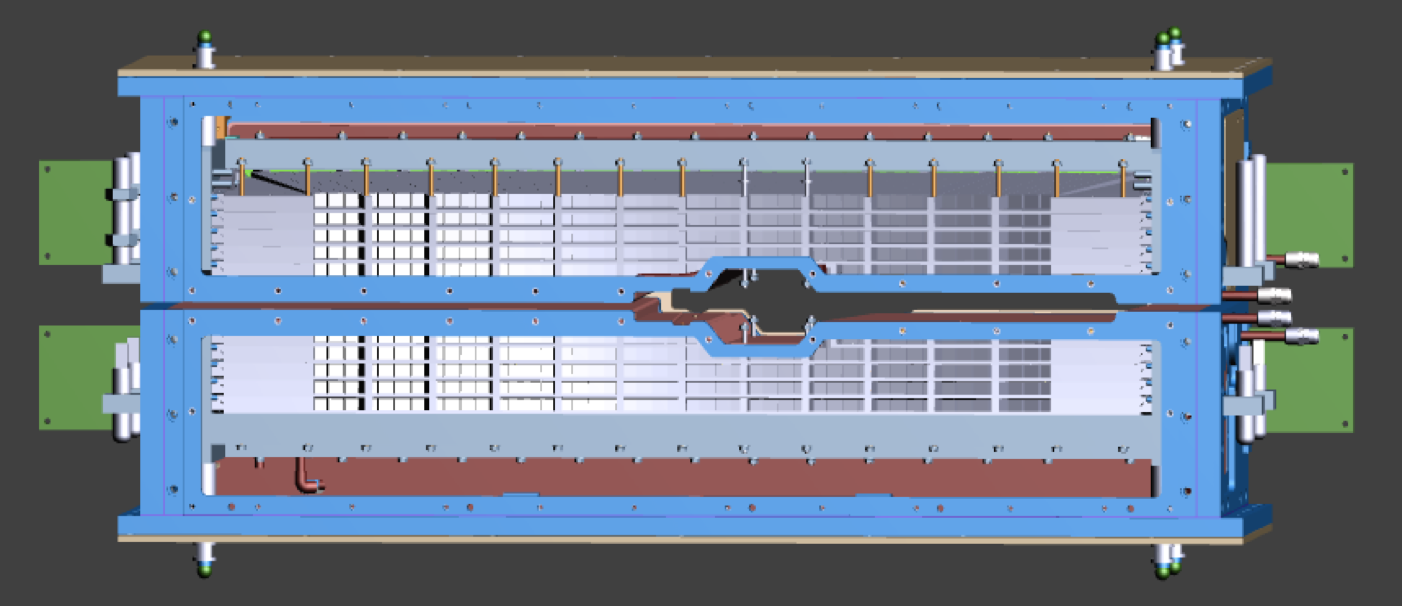
\includegraphics[width=0.85\textwidth]{pics/experiment/ecalface.png}
  \caption[Drawing of the ECal assembly face]{Drawing of the ECal assembly face, looking downstream with the beam direction. The ECal is assembled in two vertical halves and has a gap in between allowing for the electron and photon beams as well as the sheet of flame.}
  \label{Figure:ecalface}
\end{figure}

The ECal in constructed as two separate vertical halves in order to avoid the 15~mrad vertical zone of excessive electromagnetic background along the beam line. The crystals in each half are arranged in five layers of 46 crystals. The layer of crystals closest to the beam in each half has nine crystals removed to allow for the passing of the electron beam. The two halves of the ECal rest at 2~cm vertical distance from the  horizontal electron beam plane.

\begin{figure}[thb]
  \centering
      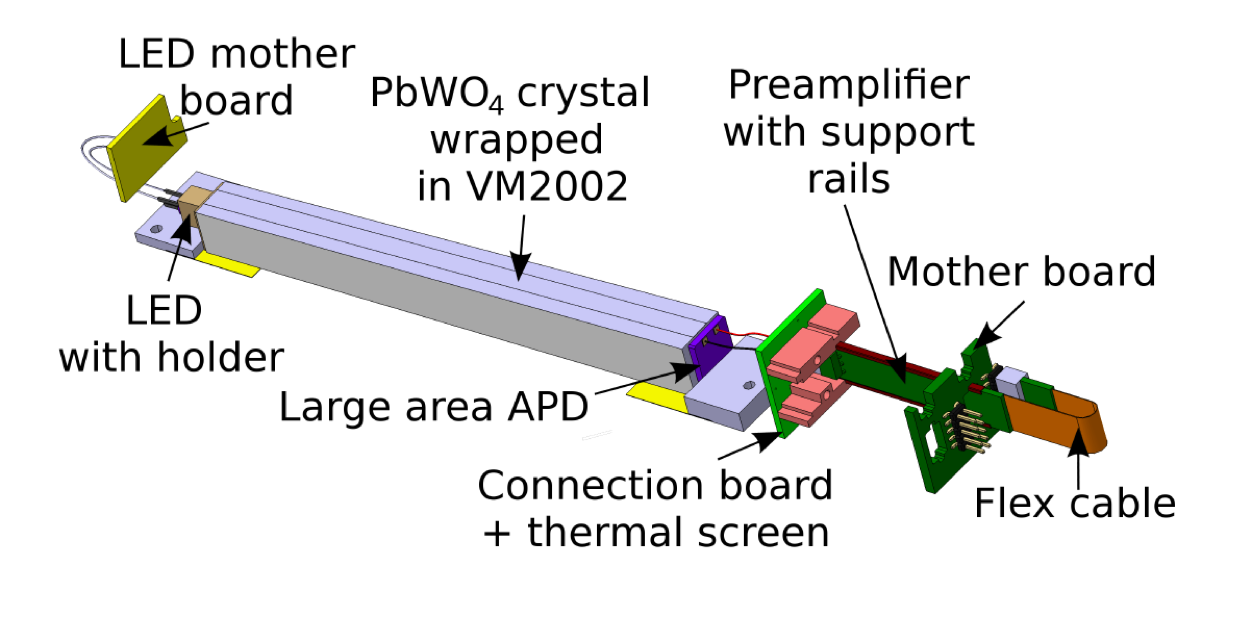
\includegraphics[width=0.85\textwidth]{pics/experiment/crystal.png}
  \caption[Single ECal module]{Drawing of an ECal crystal in readout configuration.}
  \label{Figure:crystal}
\end{figure}

Each crystal is wrapped in a VM2002 reflecting foil in order to increase light collection. The original APDs used by the the IC had a surface area of 5$\times$5~mm$^2$, but these were upgraded for HPS running by replacing each original APD with a large area APD (model S8664-1010) of surface area 10$\times$10~mm$^2$. The upgraded large area APDs are capable of collecting four times the light as compared to the same energy deposited into the old APDs. The larger signals require less electronic amplification of the signal and improve the signal-to noise-ratio. Ultimately, the upgrade in electronics requires a lower energy threshold for module readout and improves energy resolution. \\
\indent As a particle enters the ECal, it deposits all of its energy in an electromagnetic shower by either bremsstrahlung of pair production. The secondary particles then produce more particles through bremsstrahlung and photon pair production giving rise to a cascade of particles, decreasing in energy. After the electron energy is too low to yield further particles, the remaining energy is deposited through ionization and excitation releasing scintillation photons in the lead tungstate crystal that are gathered at the back of the crystal with an APD that converts the number of collected photons into an electronic signal via the photoelectric effect. Each APD is attached by a twisted pair connector to a preamplifier which converts the signal current to voltage and has low input impedence and noise.  

\begin{figure}[H]
  \centering
      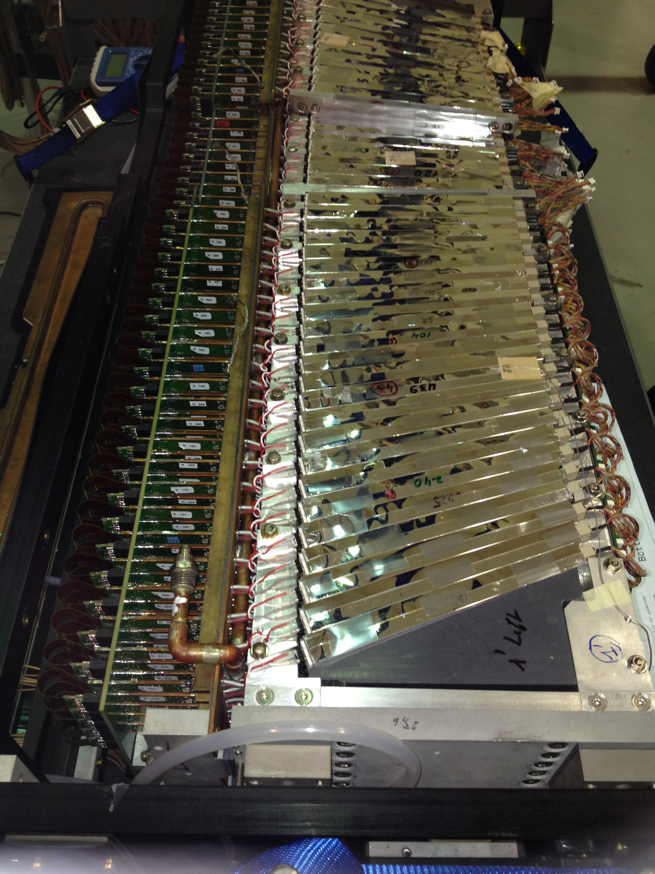
\includegraphics[width=0.5\textwidth]{pics/experiment/ecalAssembly1.png}
  \caption[Photograph of ECal crystals during assembly]{Photograph taken during assembly of the ECal from above. The preamplifiers attached to each crystal are shown on the left. As single layer of wrapped crystals are shown in their tray and the LEDs attached to each crystal are shown on the right.}
  \label{Figure:ecalAssembly1}
\end{figure}

The gain of the APDs and the scintillation of the crystals in the ECal are temperature-dependent. An Anova A-40 external chiller operating at 17$\degree$C pumps cool water through copper cooling pipes that run along the inside of the ECal at the top, bottom, front and back face of the crystal structure. The internal temperature of the ECal was monitored using sixteen thermocouples located at various locations within the ECal structure. The thermocouples are readout using an Omega D5000 series transmitters. Both devices are connected through RS-232 serial communications for external monitoring and alarms should the temperature change significantly.\\
\indent Low voltage is supplied to the preamplifiers via an Agilent 6221 operating at 5~V and approximately 4.1~A when all preamplifiers are connected. The high voltage to each of the 52 APD groups is supplied by the CAEN A1520P modules in the SY4527 mainframe. Both voltage suppliers are monitored and accessible for remote operations.  
